\chapter{Methodology} \\ \\
In this chapter the author will discuss the methodologies used to approach the project in areas such as planning, organization, development and management of the project. This section will aim to provide the reader with apt insight into how the project developed from its research stage into the final product that it is now. \\
As part of the 4 year course of Computing in Software Development a number of modules, such as Systems Analysis and Project Management, were designed to enlighten students on the different approaches or methodologies that could be taken throughout a projects development. Frequent methodologies which were taught as part of these modules were extreme programming, waterfall and RAD (Rapid Application Development). 

\section{Research Methodology} \\ \\
In the case of this project, both Qualitative Research and Quantitative 
Research were used as the approach to conducting the appropriate research. Qualitative research is an exploratory research method used to gain a greater understanding on a topic, it is also used as an aid to further quantitative research. The qualitative research was carried out by closely examining similar web based technologies to the the end goal of the project, such as Amazon, eBay and many other e-commerce based applications. It was at this point that the approach to the project in aspects such as software development methodologies were determined. \\
As the qualitative research continued a shift towards more quantitative research occurred, throughout this research a better idea of what features were commonly expected and found on web applications similar to that of the project. \\ \\

\section{Software Development Methodology} \\
The software development methodology appropriated throughout the development of this project was Extreme Programming\cite{agile}. Extreme Programming is considered to be a highly agile software development methodology that aims to produce high quality software. This methodology is noted for allowing the the development to change and adapt to the request of a client or customer. The use of this methodology in the projects development cycle was important as it, like all agile methodologies, allowed for any changes to have minimal impact on the project. \\
Shortly into the development cycle it became clear that Extreme Programming was highly appropriate in this project scenario as it allowed for the adaption to changing requirements on the advice of the project supervisor as part of the weekly stand-up meetings. As part of extreme programming features deemed to be priorities are ear-marked to be completed first, the test-driven nature of extreme programming allowed for confirmation that these features were in working order, which in turn allowed for the focus to be moved along down the priority list. \\
Further reasoning as to why this methodology was chosen was because of the amount of potential new technologies involved with the development of this project. As the author may not have had previous experience in working with some of the technologies, the full libraries and capabilities of these technologies would not be known to the author and as such the agile methodology allowed for the author to implement any features and knowledge developed throughout the project and keep the impact of any changes to a minimum. \\

\begin{figure}[h!]
	\caption{The Extreme Programming Cycle}
	\centering
	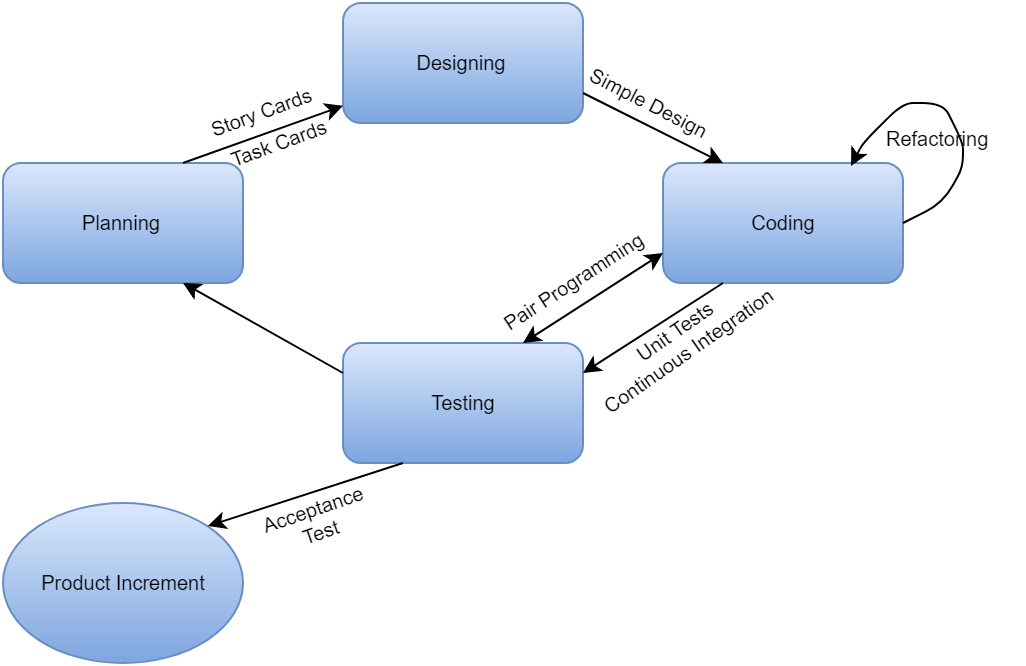
\includegraphics[width=0.9\textwidth]{images/xp}
\end{figure}

\subsection{Weekly Meetings} \\
As part of the project it was determined that participants would engage in weekly stand-up meetings with a preassigned project supervisor. In this scenario the supervisor acts as a pseudo-client, which allowed for better implementation of an agile software development methodology. The initial meetings centered on updates on a decision of a project subject, this is where the majority of the qualitative research was conducted, and whether or not this subject would be within the scope of the project statement. After the project subject had been determined the stand-up meetings mainly consisted of providing the supervisor with updates on the development process, with feedback on said updates and a discussion on what next would be implemented as part of the project. The weekly stand-up meetings can also be said to bear a strong resemblance to the stand-up meetings integrated as part of the SCRUM development methodology

\section{Development Tools} \\
In the process of developing this project two main development tools were used, Github and Visual Studio Code. Github is a web-based technology that allows for hosting of software via the command line tool git. Git is an open-source version control system that allows for changes to the project to be pushed and stored on Github. In the case of this project Github was used as the version control system as it was most familiar to the author and the tracking of progress was outlined as an important aspect of the project.\\
Visual studio code is a source code editor. In the case of this project visual studio code was chosen as it supports multiple file types like those present in an Angular based project and the integrated terminal allows for the integration of libraries that were needed throughout the projects development.



